\documentclass[a4paper,11pt]{article}

\usepackage[T1]{fontenc}
\usepackage[utf8]{inputenc}
\usepackage{graphicx}
\usepackage{xcolor}
\usepackage[T1]{fontenc}
\renewcommand\familydefault{\sfdefault}
\usepackage{tgheros}
\usepackage[defaultmono]{droidmono}
\usepackage[export]{adjustbox}
\usepackage{multirow}
\usepackage{tabularx}
\usepackage{float}
\usepackage{wrapfig}
\usepackage{amsmath,amssymb,amsthm,textcomp}
\usepackage{enumerate}
\usepackage{multicol}
\usepackage{tikz}
\usepackage[ngerman]{babel}
\usepackage{xpatch}
\usepackage[bottom]{footmisc}
\usepackage{footnote}
\usepackage{acronym}
\usepackage{float}
\bibliographystyle{unnsert}
\usepackage{geometry}
\geometry{total={210mm,297mm},
left=25mm,right=25mm,%
bindingoffset=0mm, top=20mm,bottom=20mm}


%\linespread{1.3}



% custom theorems if needed
\newtheoremstyle{mytheor}
    {1ex}{1ex}{\normalfont}{0pt}{\scshape}{.}{1ex}
    {{\thmname{#1 }}{\thmnumber{#2}}{\thmnote{ (#3)}}}

\theoremstyle{mytheor}
\newtheorem{defi}{Definition}

% my own titles
\makeatletter
\renewcommand{\maketitle}{
\begin{center}
\vspace{2ex}
{\huge \textsc{\@title}}
\vspace{1ex}
\\
\linia\\
\@author \hfill \@date
\vspace{4ex}
\end{center}
}
\makeatother
%%%

% custom footers and headers
\usepackage{fancyhdr}
\pagestyle{fancy}
\lhead{}
\chead{}
\rhead{}
\cfoot{}
\rfoot{Page \thepage}
\renewcommand{\headrulewidth}{0pt}
\renewcommand{\footrulewidth}{0pt}%%%----------%%%----------%%%----------%%%----------%%%

\begin{document}
\begin{titlepage}
	\begin{figure}
	\includegraphics[width=0.4\textwidth,right]{{logo.jpeg}}
	\end{figure}
	\centering
	{\scshape\LARGE Hochschule Esslingen\par}
	\vspace{1cm}
	{\scshape\Large Studienarbeit\par}
	\vspace{1.5cm}
	{\huge\bfseries Sirenen Erkennung durch ein Neuronales Netz\par}
	\vspace{2cm}
	{\Large\itshape Seifeddine Mhiri\par}
	\vfill
{\Large\itshape im Studiengang Technische Informatik\\
der Fakultät Informationstechnik\\
Sommersemester 2020\par}
\vspace{5cm}
{\Large\itshape ------------------------------------------------------------------- \\ 

Betreuer: 
Prof. Dr.-Ing. Thao Dang \\
  -------------------------------------------------------------------}
\end{titlepage}
\newpage

\vspace*{150px}
\noindent\huge{Eidesstattliche Erklärung}\\\\
\large{\\
Hiermit erkläre ich, die vorliegende Arbeit selbstständig und unter ausschließlicher Verwendung der angegebenen Literatur und Hilfsmittel erstellt zu haben.\\\\
Die Arbeit wurde bisher in gleicher oder ähnlicher Form keiner andern Prüfungsbehörde vorgelegt und auch nicht veröffentlicht.\\
\\Esslingen, den 1.März.2020 \hspace{2.5cm}{\_\_\_\_\_\_\_\_\_\_\_\_\_\_\_\_\_}
\\\hspace*{9.3cm}Unterschrift\\}
\vspace*{250px}
\newpage
\vspace*{150px}
\noindent\huge{Vorwort}\\\\
\large{Den Bachelor-StudentInnen für den Studiengang technische Informatik der Fakultät Informationstechnik an der Hochschule Esslingen ist es Pflicht im sechsten Semester ihres Hauptfachstudiums das Modul „Studienprojekt“ zu belegen. Ich habe mich dazu entschieden, im Rahmen eines Studienprojektes meine im Studium erworbenen Kompetenzen zu erweitern und zu vertiefen. Für die Erarbeitung eines möglichen Projektverlaufes habe ich hierzu neben den über das Institut bereitgestellten Informationen mehrere Beratungsgespräche mit meinem fachinternen Betreuer wahrgenommen. Da ich mich sehr für maschinelles Lernen interessiere und zum Zeitpunkt der Ideenfindung gerade ein Seminare über " künstliche Intelligenz und Deep learning" \space belegt habe, ordnete ich mein Studienprojekt in das Thema Sirenen Erkennung durch ein Neuronalesnetz ein.}
\newpage
\tableofcontents
\newpage
\addcontentsline{toc}{section}{Abbildungsverzeichnis}

\listoffigures
\newpage
\addcontentsline{toc}{section}{Abkürzungsverzeichnis}
\noindent\huge{Abkürzungsverzeichnis}
\\ \large
\begin{acronym}[Bash]
\acro{KI}{Künstliche Intelligenz}
\acro{KNN}{Künstliches neuronales Netz}
\acro{2D}{Zwei Dimensional}
\end{acronym}
\newpage
\section{Einführeung}
Im Zuge der Digitalisierung entstanden eine Vielzahl an neuen Möglichkeiten, klang aufzunehmen und zu verwahren. Ein Klang wird als Information im Rechner lokalisiert und verarbeitet. Um an den vollen Informationsgehalt zu
gelangen, ist es notwendig, den jeweiligen Klang zuordnen zu können.
In den letzten fünf Jahren hat sich die Entwicklung der künstlichen Intelligenz auf das Medium Klang verlagert, sei es, um neue Musikformen (mit unterschiedlichem Erfolg) zu schaffen oder um bestimmte Klangerkennung anhand von Daten zu identifizieren. 
Obwohl neuronale Netze mit langem Kurzzeitgedächtnis normalerweise mit audio-basierten Deep-Learning-Projekten verbunden sind, können Elemente der Tonidentifikation auch als herkömmliche Bildklassifizierungsaufgabe für mehrere Klassen unter Verwendung von Faltungs-neuronalen Netzen angegangen werden.
In diesem Projekt wird es gezeigt, wie ein einfaches neuronales Netzwerk, das in Keras erstellt wurde, zusammen mit einigen hilfreichen Audioanalysebibliotheken und mithilfe von verfügbarem Datensatze Sirenen Sounds mit hoher Genauigkeit erkennen kann.
\subsection{Ziel der Arbeit}
Ziel dieser Studienarbeit ist die Umsetzung eines solchen Verfahrens zur
Erkennung von Sirenen mithilfe eines künstliches neuronalen Netzes. 
Das Ergebnis soll ein Deep Learning Modell sein, das in
der Lage ist, die Sirenen Klänge in Form von WAV-Dateien möglichst genau zu erkennen. Dafür wird zunächst ein solches Verfahren implementiert und angewendet. Die Resultate des Verfahrens sollen auf ihre Qualität, sowie potentielle Schwachstellen analysiert werden. Auf Basis dieser Ergebnisse werden anschließend mögliche Verbesserungen für das Verfahren entwickelt und implementiert. Das daraus resultierende System wird
erneut auf seine Qualität getestet und mit den Resultaten des ursprünglichen
Entwurfes verglichen, um den Erfolg der Erweiterungen bewerten zu können.
\subsection{Struktur der Arbeit}
Die folgende Arbeit ist in mehrere Kapitel unterteilt, die die aufeinanderfolgenden Arbeitsschritte beinhalten. Im Grundlagenkapitel wird zunächst die Problemstellung näher betrachtet. Dazu werden anschließend die wichtigsten Begriffe geklärt, die im Verlauf dieser
Arbeit aufkommen. Es wird außerdem der Datensatz näher vorgestellt und charakterisiert sowie dargestellt und welche Tools im Projekt angewandt werden.
Abschließend wird die Zielsetzung abgegrenzt und zusammengefasst, welche Anforderungen sich aus der Analyse ergeben.\\
Im nächsten Kapitel wird die Implementierung beschrieben, nachdem man sich für ein Modell entschieden hat. Am Anfang des Kapitels werden die Daten vorgestellt und genau erklärt. Danach werden die Daten verarbeitet und aufgeteilt. Im nächsten Schritt wird das Model bereit gestellt und Trainiert. Nachdem Training kommt die Test Phase. Zum Schluss werden die Ergebnisse der Experimente zusammengefasst.
\newpage
\section{Grundlagen}
\subsection{Machine Learning}
\begin{center}
"Machine Learning is the field of study that gives computers the ability to \\ learn without being explicitly programmed. Arthur Samuel, 1959"
  \end{center}
  Der Zweck des maschinellen Lernens besteht darin, den Lernprozess zu automatisieren. Diese Aufgabe ist für den Benutzer so einfach wie möglich Gut realisiert. Aus diesem Grund sollte der Programmierer den Algorithmus nicht einstellen Verschrieben werden, aber selbst lernen ", erledige Aufgabe A so weit wie möglich "" lösen. Aufgabe A umfasst normalerweise das Aufrufen einer bestimmten Eingabe produziere eine bestimmte Ausgabe. Die Eingabe ist Haben spezifische Eigenschaften (wie Vektor oder eine Matrix aus mehreren Zahlen oder ein Satz aus mehreren Wörtern). Die beiden wichtigsten gemeinsamen Aufgaben sind Regression und Klassifizierung.
Wie in Abbildung 1 gezeigt wird, ist künstliche Intelligenz eine Reihe von Software und Programme, die Probleme allein Lösung können. Machine Learing ist hier ein Teil der KI und der Algorithmus die von Daten lernen können \cite{machine}.
Die Daten werden können mit einem Einsatz von tiefen neuronalen Netzen verwendet werden.
  \begin{figure}
	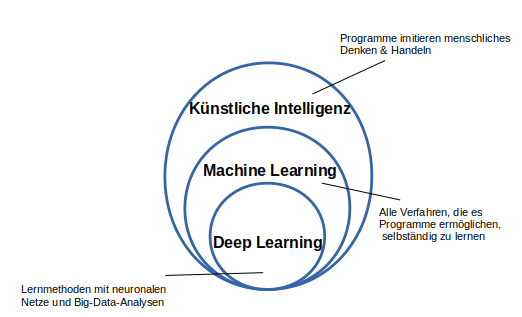
\includegraphics[width=1\textwidth]{MachineLearning.png}
	\caption{Darstellung Machine Learning}
	\end{figure}
\subsection{Deep Learning}
Deep Learning ist ein Teilbereich des maschinellen Lernens, bei dem neuronale Netze und große Datenmengen verwendet werden. Die Lernmethode hängt von der Funktionsweise des menschlichen Gehirns ab und kann eigene Vorhersagen oder Entscheidungen treffen. Deep Learning verwendet neuronale Netze mit Basis von vorhandener Informationen. Trainingsmethoden, die große Datenmengen verwenden und analysieren, können zur Erzeugung künstlicher Intelligenz verwendet werden. Deep Learning eignet sich besonders für alle Anwendungen, aus denen große Datenmengen zu Mustern und Modellen abgerufen werden können. Künstliche neuronale Netze sind die technische Grundlage des tiefen Lernens und werden während des Lernprozesses wiederholt miteinander verbunden  \cite{deep}.\\
Häufige Anwendungsfälle für Deep Learning sind Bild- und Spracherkennung, prädiktive Analysen, Empfehlungssysteme oder Anomalieerkennung.
Im Vergleich zu anderen maschinellen Lernprozessen ist Deep Learning sehr kompliziert. Trotzdem lohnt sich der Aufwand insbesondere im wirtschaftlichen Umfeld. Aber wie führt man am besten Deep-Learning-Projekte durch? Der Schlüsselfaktor für den Erfolg ist die maximale Menge an qualitativ hochwertigen Daten, die zum Trainieren neuronaler Netze verwendet werden. Bei der Bilderkennung erfordern die automatische Merkmalsextraktion und das Training Tausende von Bildern. Aufgrund der großen Datenmenge kann das Training von Deep-Learning-Modellen lange dauern. Normalerweise wird das Netzwerk generiert, indem eine große Datenmenge über das Problem gesammelt und anschließend die Architektur und das Modell entworfen werden, um die erforderlichen Funktionen zu erlernen. Im Allgemeinen können Frameworks und Tools wie TensorFlow oder Torch verwendet werden, um Deep-Learning-Modelle und -Architekturen zu entwickeln. Da es sich in der Regel um Open Source handelt, können interessierte Entwickler problemlos darauf zugreifen.
Ein einfaches künstliches neuronales Netz besteht aus ein Input Layer (Eingangsschicht), ein Hidden Layer (versteckten Schicht) sowie ein Output Layer (Ausgangsschicht). Die Neuronen im Hidden Layer enthalten sogenannte Gewichte und verteilen die Ausgabeergebnisse auf verschiedene Eingangssignale. Dabei werden Input-Signale über Aktivierungsfunktionen gesichtet und transformiert. Wie man in Abbildung 2 sehen kann, können neuronale Netze beliebig komplex sein. Beispielsweise kann ein einfacher KNN nur eine verborgene Schicht haben, während die komplexere Methode nur 100 verborgene Schichten hat. Wenn man über Deep Learning spricht, bezieht man sich auf Modelle, die mehrere versteckte Schichten haben müssen\cite{deep2}.
Deutlich komplexer sind Convolutional Neural Networks (CNNs), zu Deutsch:
neuronale Faltungsnetzwerke. Man hat maßgeblich zum Aufschwung bei der
Bilderkennung beigetragen.


\begin{figure}
	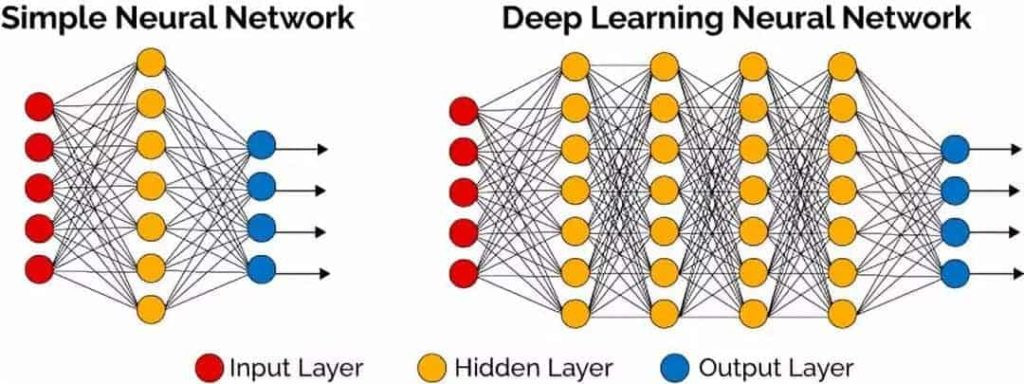
\includegraphics[width=1\textwidth]{deep-learning.jpg}
	\caption [Diagramm eines Deep Neural Networks]{Diagramm eines Deep Neural Networks Diagramm eines Deep Neural Networks}
	\end{figure}
	\footnotetext{Quelle: [Online] https://datasolut.com/was-ist-deep-learning/}
	
\subsection{Convolutional Neural Networks (CNN)}
Bei den Convolutional Neuronal Networks (CNN oder ConvNets) "Faltungsnetzwerke" ist ein tiefes Lernen Technik, die aus mehreren Schichten besteht. ConvNets wurden in einer Vielzahl von Anwendungen verwendet, wie z.B Bildklassifizierung, Objekterkennung, Spracherkennung, Verarbeitung natürlicher Sprache und medizinische Bildanalyse. Convolutional Neuronale Netze sind Computer Vision mit vielen Verwendungsmöglichkeiten, bei denen die Hauptkonzepte von ConvNets beibehalten, übergeordnete lokale Funktionen aus Eingaben (normalerweise Bilder) eingegeben und zu komplexeren Funktionen kombiniert werden Funktioniert auf der unteren Ebene. Aufgrund seiner mehrschichtigen Architektur ist es jedoch rechenintensiv und das Trainieren solcher Netzwerke in einem großen Datensatz dauert mehrere Tage. Daher werden solche tiefen Netzwerke normalerweise auf GPUs trainiert. CNN sind bei visuellen Aufgaben so leistungsfähig, dass sie besser abschneiden fast alle herkömmlichen Methoden\cite{CNN}.\\
\begin{displaymath}
(f*g)(n) = \sum_{m} f(m)g(n-m)
\end{displaymath}
Der Konventionale-Operation ist einer der wichtigsten Vorgänge für digitale Signale. Er wird in vielen Bereichen verarbeitet und verwendet, einschließlich Statistik, Wahrscheinlichkeit, Sprachverarbeitung, Computer Vision und Bildverarbeitung. Es kann auch auf höherdimensionale Funktionen angewendet werden. Hier kann man zweidimensionale Funktionen verwenden. Ein Beispiel dafür wäre, zweidimensionaler Filter, zweidimensionale Eingabe und die zweidimensionale Feature-Map, die in Folgende Abbildung dargestellt sind. Ein zweidimensionales Bild wird als input wird mit A bezeichnet. Ein 2D Filter mit m und n als Größen wird mit K bezeichnet. Die 2D feature map wird mit F bezeichnet. A wird mit K gefaltet und erzeugt F. Daraus folgt:
\begin{displaymath}
F(i,j) = (A*K)(i*j)= \sum_{m} \sum_{n} A(m,n)K(i-m, j-n)
\end{displaymath} 
Die Operation ist kommutativ und der Kernel K wird relativ zur Eingabe gespiegelt. Wenn der Kernel nicht gespiegelt ist, dann
Die Faltungsoperation ist dieselbe wie die unten angegebene cross-correlation. Diese Methode wird von vielen CNN Bibliothek benutzt. Die Gleichung ist:
\begin{displaymath}
F(i,j) = (A*K)(i*j)= \sum_{m} \sum_{n} A(m+i, n+j)K(m, n)
\end{displaymath}
Ein Convolutional Neural Network ist ein teilweise lokal verbundenes neuronales Feedforward-Netz, welches zu allermeist aus folgenden Schichten zusammengesetzt ist:
\begin{itemize}
\item Convolutional layer,
\item Activation function layer (ReLU),
\item Pooling layer,
\item Fully connected layer 
\item Dropout layer.
\end{itemize}
Es wird detaillierter auf die einzelnen Schichten eingegangen.\\
\textbf{Convolution layer}: Die Faltung ist die erste Ebene, die Features aus einem Input extrahiert. Die Funktion der Konvolutions schichten basiert auf der Verwendung von sogenannten Filtern, die kleine Bereiche des Eingabebildes abdecken. Breite und Höhe der Abdeckung sowie die gesamte Tiefe. Diese Filter bewegen sich über das Bild und bilden das Skalarprodukt. Ein zweidimensionaler Satz von Aktivierungen zwischen dem Filter und den Bildbereichen. Es wird mehrere Filter dieses Typs geben überlappen und so wieder dreidimensionale Ausgabe erzeugen.
\\ \textbf{Activation function layer (ReLU): }ReLU steht für Rectified Linear Unit für eine nichtlineare Operation. Die Ausgabe ist ƒ (x) = max (0, x). ReLUs sind wichtig, weil die das Ziel haben Nichtlinearität in ein CNN einzuführen. Ein ConvNet sollen nicht Negative und lineare Werte lernen. Die ReLU-Aktivierungsfunktion hat einige gewonnene
Bedeutung in den letzten Jahren und ist derzeit die beliebteste Aktivierungsfunktion
für tiefe neuronale Netze. Neuronale Netze mit ReLU trainieren viel schneller als andere.\\
\\ \textbf{Pooling layer: }Wenn das Bild zu groß ist, reduziert der Abschnitt "Pooling layer" die Anzahl der Parameter. Es gibt 3 verschiedene Art von Pooling. Das Max Pooling übernimmt das größte Element aus der korrigierten Feature-Map. Das größte Element zu nehmen, könnte auch das Average Pooling bedeuten. Die Summe aller Elemente in der Feature-Map wird als Summ Pooling aufgerufen.\\
\\ \textbf{Fully connected layer: }Die Matrix wird zu einem Vektor konvertiert  und ein neuronales Netzwerk in eine fully connected layer eingespeist. In "fully connected layer" jedes Neuron von der vorherigen Schicht (Faltungsschicht oder Pooling-Schicht oder vollständig verbundene Schicht) ist verbunden mit jedem Neuron in der nächsten Schicht und jeder Wert trägt zur Vorhersage bei wie stark ein Wert einer bestimmten Klasse entsprichtDer output von dem letzten fully connected layer wird einem Klassifikator zugeführt, der Punkte an die Klasse ausgibt.\\
\\ \textbf{Dropout layer: }Eine Dropout-Schicht kann eingeführt werden
in dem Modell, in dem einige Neuronen zusammen mit ihren Verbindungen zufällig sind während des Trainings aus dem Netzwerk entfernt. Dropout layer reduziert sich merklich Überanpassung und verbessert die Verallgemeinerung des Modells.
\begin{figure}
	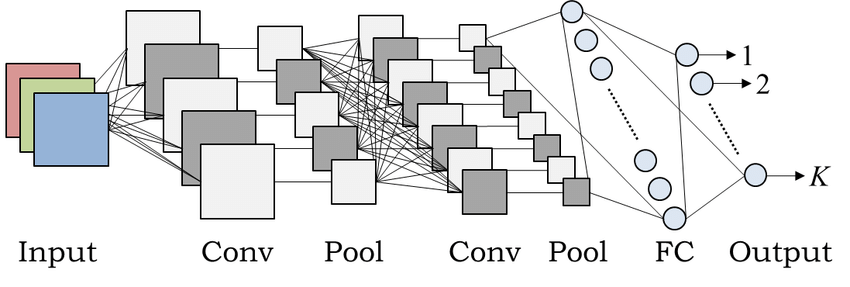
\includegraphics[width=1\textwidth]{An-example-of-CNN-architecture.png}
	\caption [Diagramm CNN-Architekturen] {Diagramm CNN-Architekturen \footnotemark}
	\end{figure}
	\footnotetext{Quelle: [Online] https://www.researchgate.net/figure/An-example-of-CNN-architecture}

\subsection{Aufbau digitaler Wavelet-Audiosignale}
Um ein grundlegendes Verständnis der Daten zu erhalten, mit denen man mich befassen werde, muss man auf eine grundlegende Ebene gehen und die Frage stellen "was ist ein Ton und wie wird er digitale übersetzt?"\\
Das Geräusch sind Kompressionen und Verdünnungen in der Luft, die ein Ohr aufnimmt. Der Klang ist eine Luftbewegung. Wird oft in einer Wellenform ausgedrückt, die zeigt, was mit Luftpartikeln passiert, die sich im Laufe der Zeit hin und her bewegen. Bei der Klassifizierung von Audio wird in der Regel eine Form von Fourier Transformation angewendet. Ein Audiosignal wird grundsätzlich in ein dreidimensionales Bild umgewandelt. Die x-Achse wird als Zeit interpretiert. Die y-Achse repräsentiert die Frequenz im Diagramm. Und schließlich werden die entsprechende Farbe Horizontal oder Ablenkung der entsprechenden Pixelfrequenz des Bildes Zu diesem Zeitpunkt als dritte Achse bezeichnet. 
\begin{figure}
	\centering
	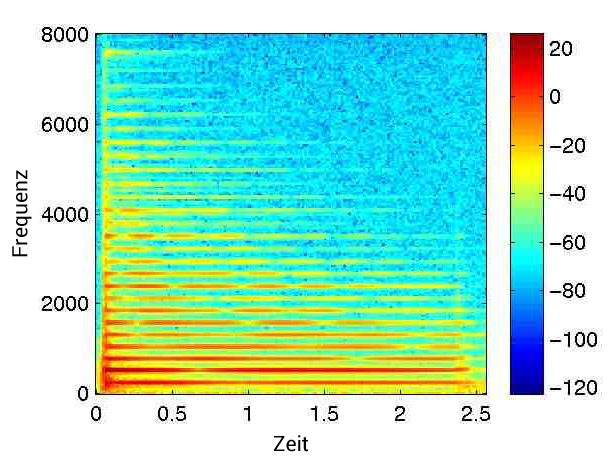
\includegraphics[width=0.5\textwidth]{spectrogram.png}
	\caption [Spectogramm eines Audiosignals] {Spectogramm eines Audiosignals \footnotemark}
	\end{figure}
	\footnotetext{Quelle: [Online] https://www.matheretter.de/wiki/shazam-spektrogramm}
In dieser Arbeit hingegen werden die Audiosignale in ihrer ursprünglichen Wavelet-Form (siehe Abbildung) analysiert und
antrainiert. Eine Wavelet-Form ist im Grunde die digitale Übersetzung eines
physischen Tons. Die Wavelet-Form ist grundsätzlich physischer Klang. Durch die A / D-Umwandlung von Ton, abgetasteter Schallwellenpegel.  Ein Scan wird als Sample bekannt, erfolgt dies Schritt für Schritt durch Audio Audiomaterial hat einen Frequenzbereich von 32 bis 96 kHz pro Sekunde. Standard der binären Abtastrate der digitalen-Audiosignale beträgt aufgrund dieser Rate 44,1 kHz (CD-Qualität) maximale Tonhöhenfrequenz, die abgetastet werden mehr als die Hälfte ist ungefähr 22 kHz, also die Frequenz. Das Spektrum des menschlichen Gehörs kann reproduziert werden. Jeder Abtastwert ist die Amplitude in einem bestimmten Zeitintervall, wobei die Bittiefe den Detaillierungsgrad des Abtastwerts bestimmt, der auch als dynamischer Bereich des Signals bezeichnet wird (normalerweise 16 Bit, was bedeutet, dass der Amplitudenbereich eines Abtastwerts 65.536 betragen kann) \cite{Abtast}.
\begin{figure}[htbp]
\begin{minipage}[c]{0.5\textwidth}

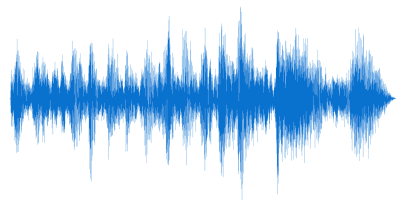
\includegraphics[width=\textwidth]{Wavelet.png}
	\caption {Wavelet-Form eines Audiosignals }
\end{minipage}
\hfill
\begin{minipage}[c]{0.5\textwidth}
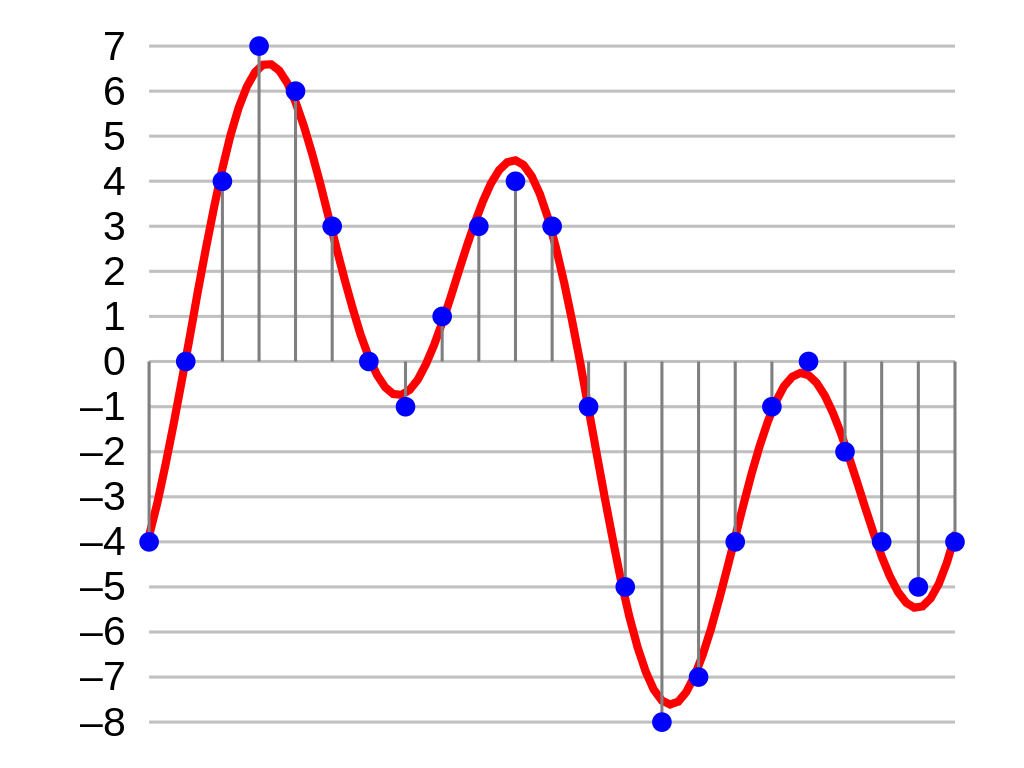
\includegraphics[width=\textwidth]{4-bit-linear-PCM.png}
	\caption [Schaubild für die Sampling-Rate eines Signals] {Schaubild für die Sampling-Rate eines Signals \footnotemark}

\end{minipage}	
\end{figure}	
	\footnotetext{Quelle: [Online] https://en.wikipedia.org/wiki/Audio\textunderscore bit \textunderscore depth}
\section{Technische Analyse}
Im folgenden Kapitel werden einige technische Grundlagen und Basistechnologien zum Thema Sirenen Erkennung durch ein Neuronales Netz allgemein erläutert. Es werden genau die benötigte Sprache mit deren Bibliotheken zum Thema Audio Verarbeitung und Deep Learning. Die Funktion der Faltungsschicht basiert auf Der sogenannte Filter, dh ein kleiner Bereich des Eingabebildes Die Breite und Höhe der Abdeckung und die gesamte Tiefe. Diese Filter bewegen sich auf dem Bild, um ein aktiviertes zweidimensionales Array zu bilden, indem sie das Skalarprodukt zwischen dem Filter und dem Bildbereich berechnen. Es wird mehrere solcher Filter geben, um wieder eine 3D-Ausgabe zu generieren.
\subsection{Python}
Python wird oft als High-Level-Allzweck-Programmiersprache bezeichnet. Die Rechte an Python liegen bei der Python Software Fundation , doch ist die Sprache offen und die Entwicklung ist kollaborativ. Es ist eine universelle, höhere Programmiersprache die objektorientiert, aber auch funktional geschrieben werden kann. \\
Aufgrund seiner einfachen Syntax und großen Flexibilität ist Python eine der am häufigsten verwendeten Programmiersprachen und gilt als Standard in den Bereichen Datenwissenschaft und maschinelles Lernen (insbesondere Deep Learning). Python bietet eine Vielzahl von Bibliotheken und Tools auf dem Gebiet der Datenwissenschaft, wie Panda, Matplotlib, Seaborn, Scikit-Learn und Numpy, um eine umfangreiche Data Science-Community aufzubauen.\\
Mit Keras, Tensorflow und Pytorch bietet Python die meisten maschinellen und Deep-Learning-Bibliotheken, die von großen Unternehmen wie Google und Facebook entwickelt und verwendet werden. Man ist der festen Überzeugung, dass Python es ermöglicht, auf relativ einfache Weise in das Gebiet der künstlichen Intelligenz einzusteigen und schnell Produktionsergebnisse zu erzielen, wodurch neue kulturelle Projekte realisiert werden.\\
Für die Audio-Analyse und-Verarbeitung in Python, wird die Bibliothek LibROSA benötigt.LibROSA bietet die Realisierung verschiedener allgemeiner Funktionen, die im gesamten Bereich des Abrufs von Musikinformationen verwendet werden. In diesem Dokument wird ein kurzer Überblick über die Bibliotheksfunktionen sowie eine Erläuterung der Entwurfsziele, Softwareentwicklungspraktiken und Symbolkonventionen gegeben.
\subsection{Jupyter-notebook}
Jupyter-Notebooks sind im Bereich der Data Science sehr beliebt und daher auch nützliche Werkzeuge für den digitalen Universitätsunterricht. Mit Jupyter Notebook können Sie interaktive "Arbeitsblätter" erstellen. Jupyter-Notebook ist eine webbasierte Umgebung, die die Erstellung, Dokumentation und gemeinsame Nutzung von Präsentatoren unterstützt, insbesondere im Bereich der Datenanalyse. Das Besondere an Jupyter Notebook ist, dass der Code und die Codebeschreibung in separaten Zellen geschrieben sind, sodass Sie separate Codeblöcke separat ausführen können. Jupyter-Notebooks können Text und Medien verwenden, einschließlich Bilder, Grafiken und Videos sowie Quellcode. Der Quellcode kann direkt ausgeführt werden \cite{Jupyter}.
Im Modul für maschinelles Lernen wird Jupyter-Notebook verwendet, um große Datenmengen zu visualisieren, zu bereinigen und auszuwerten. Insbesondere in der Wissenschaft werden verschiedene Arten von Daten generiert, darunter Zeitlimitdaten, Raum-Zeit-Daten und Bilder. Einer der großen Vorteile von Jupyter-Notebooks besteht darin, dass man komplexe Aufgaben besser aufteilen kann. Jupyternotebook eignet sich sehr gut für die Ausführungen von Python-Skripts.
\subsection{Tensorflow und Keras}
Tensorflow wurde am 09.November.2015 als Open Source Projekt
von Google veröffentlicht. Das Framework ist plattformunabhängig, was die Software leistungsfähig und gut skalierbar macht. Das Training des NN war somit leicht auf einen leistungsstarken Server zu exportieren. Gleichzeitig ist die Komplexität sehr umfangreich, was für Einsteiger suboptimal ist.\\
Keras hingegen ist eine High Level API für Deep learning, die unter anderem auf Tensorflow ausgeführt werden kann. Es wurde mit dem Ziel entwickelt, schnelles Experimentieren zu ermöglichen. Das Speichern der trainierten Modelle und das einfache Wiederverwenden dieser, macht Keras sehr interessant für diese Arbeit.\cite{Keras} 
\\ mit Keras hat man die Möglichkeit:
\\-Daten bereitstellen, bevor man das Modell trainieren.
\\-Daten vor verarbeiten und zu spalten.
\\-Ein Modell erstellen, um Ihre Daten in nützliche Vorhersagen umzuwandeln.
\\-Das Modell zu trainieren unter Berücksichtigung von Kontrollpunkten, Überwachung und Fehlertoleranz.
\\-Das Modell zur bewerten basierend auf Testdaten und wie man daraus neue Daten ableitet.

\subsection{Datensatz}
Der Datensatz, der 8732 markierte Audiodateien enthält Waveform Audio Files (WAVE) enthält und gegründet von der York University (NYU). Diese sind in zehn unterteilt Für verschiedene Kurse beträgt die Dauer jedes Kurses nicht mehr als vier Sekunden. Die Audiodatei ist nummeriert und im Datensatz enthalten. Andere CSV-Dateien, die zehn Kategorien zugeordnet sind. Diese Klassen sind "Klimaanlage", "Autohupe", "spielende Kinder", "Hundebellen", "Bohren", "Motorleerlauf", " Schuss", "Jack Hammer", " Sirenen" und " Straßenmusik". Der Datensatz ist in Trainingsdateien unterteilt (5435 Dateien) und Testdateien (3297).
\newpage
\section{Implementierung}
In weiten Teilen bezieht sich die Implementierung auf das Notebook
von Seifeddine Mhiri auf Github.
Der Verständlichkeit wegen, wird in diesem Kapitel nur
auf die wichtigen Teile der Implementation eingegangen, wobei
der komplette Programmiercode im Anhang zu finden ist.
\subsection{Step 1: Data Exploration and Visualisation}
Am Anfang werden die Basic Bibliothek installiert und aufgerufen.
Pandas- und Numpy-Softwarepakete importiert, um  die grundlegendste Datenstruktur in den meisten Algorithmen für maschinelles Lernen zu verwalten. Es bietet leistungsstarke, benutzerfreundliche Struktur- und Datenanalysetools. Als Nächstes importieren man die erforderliche Keras-Bibliothek, um unser Netzwerk und andere notwendige Hilfssoftwarepakete aufzubauen. Besonders hervorzuheben ist das Garbage Collector-Paket, mit dem man den RAM während der Datenkonvertierung bereinigen können. Schließlich hat man auch ein Arbeitsverzeichnis eingerichtet, um die konvertierten Bilder zu speichern. 
\begin{figure}[htbp]
\begin{minipage}[c]{0.5\textwidth}

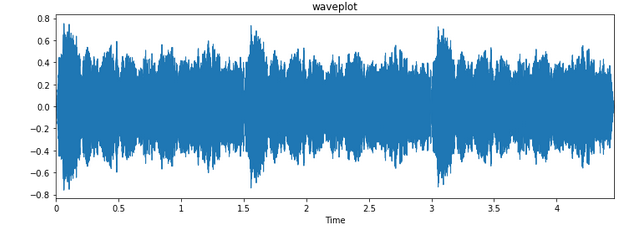
\includegraphics[width=\textwidth]{waveplot.png}
	\caption {Waveplot of Sirene
 }
\end{minipage}
\hfill
\begin{minipage}[c]{0.5\textwidth}
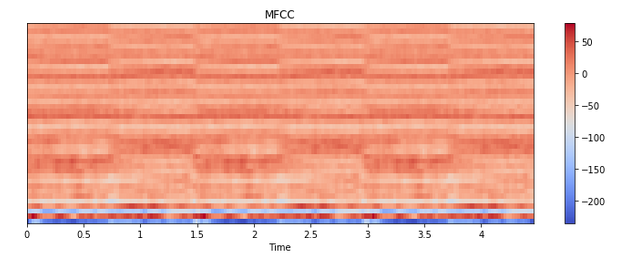
\includegraphics[width=\textwidth]{MFCC.png}
	\caption {MFCC of Sirene}

\end{minipage}	
\end{figure}	

\begin{figure}[htbp]
\begin{minipage}[c]{0.5\textwidth}

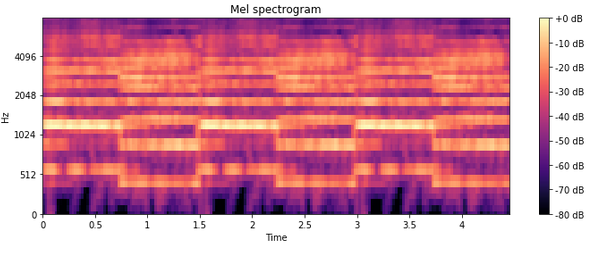
\includegraphics[width=\textwidth]{Melspectrogram.png}
	\caption {Melspectrogram of Sirine }
\end{minipage}
\hfill
\begin{minipage}[c]{0.5\textwidth}
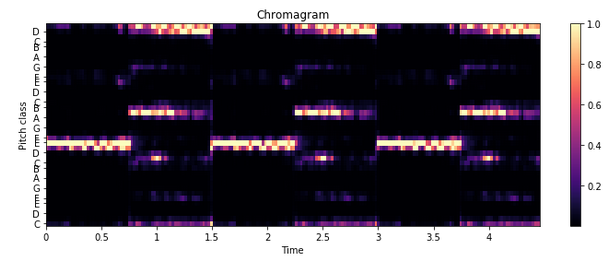
\includegraphics[width=\textwidth]{Chromagram.png}
	\caption{Chromagram of Sirine}

\end{minipage}	
\end{figure}	
Im ersten Schritt nach dem Import der benötigten Pakete werden die
Daten geladen. Als Visualisierung von Audio Dateien, wird eine Sirenen Ton als WAV-File dargestellt. In den Folgenden Abbildungen wird die Darstellung von dem Sirene.wav in 4 verschneiden arten:
\\\textbf{-Waveplot} : Zeichnen Sie die Amplitudenhüllkurve der Wellenform.
\\\textbf{-MFCC:} In der Klangverarbeitung ist das Mel-Frequenz-Cepstrum (MFC) eine Darstellung des kurzfristigen Leistungsspektrums des Schalls, das auf der linearen Kosinustransformation des logarithmischen Leistungsspektrums in der nichtlinearen Mel-Reihenfolge basiert.
\\\textbf{-Melspectrogram:} ist ein Spektrogramm mit der Physikalische Einheit Mel Skala.
\\\textbf{-Chromagram:} ist ein Spektrogramm mit Farbsättigung als Eigenschaft.
\\\\Durch visuelle Inspektion kann man erkennen, dass es schwierig ist, die Unterschiede zwischen bestimmten Klassen zu visualisieren. Insbesondere sind die Wellenformen für Wiederholungstöne.
Das menschliche Ohr kann natürlich den Unterschied zwischen den Harmonischen erkennen. Es wird interessant sein zu sehen, wie gut ein Deep-Learning-Modell in der Lage ist, die notwendigen Merkmale zur Unterscheidung zwischen diesen Klassen zu extrahieren.
\subsection{Step 2: Data Preprocessing and Data Splitting}
Der nächste Schritt besteht darin, die Funktionen zu extrahieren, die zum Trainieren des Modells erforderlich sind. Zu diesem Zweck erstellen wir eine visuelle Darstellung jedes Audio-Samples, anhand derer wir die zu klassifizierenden Merkmale mit denselben Techniken identifizieren können, mit denen die Bilder mit hoher Präzision klassifiziert werden.
Das Spektrogramm ist eine nützliche Technik, mit der das Frequenzspektrum von Schall und seine Veränderungen in sehr kurzer Zeit visualisiert werden können. Man wird Melspectrogram verwenden.
Der UrbanSound-Datensatz enthält 8732 kurze (weniger als 4 s) Klangausschnitte von Stadtlärm, die als 10 verschiedene Kategorien gekennzeichnet sind. Das Trainings- und Testdatensätze bestehen aus WAV-Dateien und zugehörigen CSV-Tabellen, die eine korrekte Beschreibung der ID und der Trainingsdaten enthalten, die als Beschriftungen verwendet werden. Um die Daten in eine Spektrogrammdarstellung umzuwandeln, verwenden man die Bibliothek LibROSA. Als Nächstes beginnen man mit der Datenkonvertierung, indem man die Funktionen definieren, mit denen die WAV-Dateien in Bilder im JPG-Format konvertiert werden. Kurz erklärt, extrahieren man die Audio-Zeitreihen und die Abtastrate jeder .wav-Datei mit LibROSA, bevor man ein Spektrogramm der Daten erstellt, plotten und als entsprechendes Bild speichern. 
Sobald alles definiert mit der Funktionen "create\textunderscore spectrogram" 
, "create\textunderscore spectrogram\textunderscore test" ist, werden die Trainingsdaten transformiert. 
Es werden die Stapelverarbeitung von 2000 Bildern verwenden, um diese Vorgänge gleichzeitig abzuschließen, und das Garbage Collector-Paket verwenden, um die Speichernutzung zwischen Stapeln zu optimieren.
Im Gegensatz zu unserem vorherigen Lernprogramm befindet sich Datenbezeichnung nicht direkt im Dateinamen des Bildes im Projekt, sondern in der zugehörigen CSV-Tabelle. Keras bietet jedoch einen einstufigen Datengenerator, mit dem das richtige Etikett im Arbeitsblatt leicht gelesen und die Daten in bestimmten Stapeln für Training und Validierung verarbeitet werden können. Der Datengenerator benutzt die Dataframes von den CV-Dateien und die Bilder der Trainingsdateien. Der "batch size" definiert die Anzahl der Proben, die über das Netzwerk verbreitet werden. Der "Target size" ist die Größe des Bild und repräsentiert 64 breite und 64 Länge.
\subsection{Step 3: Model Training and Evaluation}
\subsubsection{Model vorbeireiten und  aufsetzen}
Der nächste Schritt wird darin bestehen, diese Datensätze zu verwenden, um tiefe neuronale Netze aufzubauen und zu trainieren und Vorhersagen zu treffen. die Netzwerkarchitektur besteht aus 6 Layers mit zunehmender Filterdichte, um die Merkmale jedes Bildes jeder aufeinanderfolgenden Schicht am besten zu extrahieren. Die zusammengeführte Schicht und die fehlende Schicht werden verwendet, um die Berechnungseffizienz zu verbessern bzw. eine Überanpassung zu verhindern.
Bei unseren Versuchen wurde beobachtet, dass das Hinzufügen von Schichten mit einer hohen Anzahl von Filtern am Ende des Netzwerks die Genauigkeit um bis zu 12\% erhöhen kann. Intuitiv kann dies als ein früherer Ebenenfilter verstanden werden, dessen Ziel es ist, Merkmale zu teilen, die grundsätzlich von allen Spektrogrammen (Linie und Kurve) gemeinsam genutzt werden. Umgekehrt sind die Spektrogramme, sobald man die späteren Schichten und ihre Faltungsausgangsgrafen erreicht haben, so ähnlich, dass eine größere Anzahl komplexer Filter besser zur Unterscheidung beiträgt. Man kann die Netzwerkarchitektur jederzeit ändern, um diese Informationen aus erster Hand zu verstehen.\\

Für den Aufbau des CNN-Models wird wie in Kapitel 2.3 bereits erwähnt, eindimensionale CNN-Schichten genutzt mithilfe der Keras API das Modell des CNNs gebaut. Es werden die benötigten Bibliotheken für ein CNN Aufbau importiert. In Zeile 8 wird der erste Layer hinzugefügt. Dabei steht „Conv2D“ für einen Convolutional-Layer. Die 32 steht für die Anzahl der Output-Filter und das Argument „(3,3)“ für die Kernel Größe. Das Argument „padding“ legt in diesem Fall „same“ gewählt wurde. Dies bedeutet, dass überstehende Werte bei der Faltung ersatzlos gestrichen werden und durch Padding kein weiteres Feld
mit hinzugefügten Werten erzeugt wird. In Zeile 10 wird als
Aktivierungsfunktion die lineare ReLU-Funktion festgelegt. Diese legt fest, aufgrund welcher Funktion ein Neuron im Netz aktiviert wird. In Zeile 13 wird nun das Pooling durchgeführt und in Zeile 14 wird als Aktivierungsfunktion die lineare ReLU-Funktion festgelegt. Mit Zeile 16 wird einer Überanpassung, „Dropout“ genannt, des Netzes entgegengewirkt. Von Zeile 11 bis 24 werden die restlichen 5 Layers definiert. Zwischen der Faltungsschicht und der vollständig verbundenen Schicht befindet sich eine "Flatten" Schicht. Durch das Reduzieren wird eine zweidimensionale Matrix von Merkmalen in einen Vektor konvertiert, der in einen vollständig verbundenen Klassifizierer für neuronale Netze eingegeben werden kann. In Zeile 29 wird die letzte Schicht hinzugefügt. Diese ist exakt so
groß gewählt, dass als Ergebnis nur eine der Klassen des Datensatzes herauskommen kann. Das bedeutet, das Netz entscheidet sich immer für eine Klasse des Datensatzes. Hierbei wird als Aktivierungsfunktion die „softmax“-Funktion eingesetzt. Diese gibt die Wahrscheinlichkeit an, dass eine der Klassen wahr ist.
\subsubsection{Model Trainieren}
Es werden am Anfang die Step Size von dem Training und der Validierung definiert. Mit dem Befehl "Model.fit" wird das Model trainiert, indem die benötigten Parameter eingebt. Es werden hier 150 Epochs gesetzt. Mehrere Epochs bedeuten, dass mehrere Trainingseinheiten absolvieren müssen. Das Model wird als Generator evaluiert und ein Score wird kalkuliert. Diese Score gebt das "Training Accuracy" ab. Das Training wird gespeichert mit der "save" Funktion. Danach kommen die Ergebnisse des Trainings. Wie in der folgenden Abbildungen wird die Accuracy Kurve Links und Rechts wird die Loss Kurve gezeigt. In Abbildung 11 ist die Genauigkeit des Netzes zu sehen. Die Genauigkeit des Netzes,
getestet mit den Daten aus der Validation, beträgt 93\%. Grundsätzlich sind knapp 97\% positiv
zu bewerten und für einige Anwendungsfälle ist optimal.
besonders bei zunehmender Epochenanzahl (vgl. Abbildung 11)
\begin{figure}
	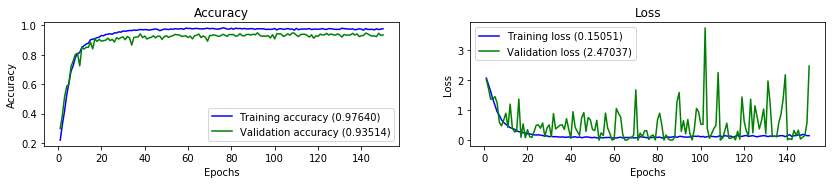
\includegraphics[width=1\textwidth]{rechts.png}
	\caption [Accuracy and loss Training/Validation Diagram] {Accuracy and loss Training/Validation Diagram}
\end{figure}


\subsection{Step 4: Testing}
Es scheint, dass das erzeugte Modell mit einer Genauigkeit von nahezu 95\ recht gut zu den Daten passt. Dieses Projekt demonstriert die inhärente Leistungsfähigkeit guter, sauberer und gekennzeichneter Daten. Wenn man das Netzwerk nur mit einem Bruchteil der Trainingsdaten betreiben, beispielsweise mit den ersten 1500 Bildern. Dies hängt mit der Ähnlichkeit unserer Spektrogramme zusammen.
Wie in den Trainingsdaten werden auch die Testdaten in Form von "jpg" Dateien umgewandelt. 
Ein Testgenerator wird über Dataframe aufgesetzt. Steps von Tests werden generiert. Es sind 103 Steps in unserem Test. Es gibt Bilder mit 10 Klassen. Man verwendet den Predictgenerator, um die Wahrscheinlichkeiten von Bildern mit mehreren labels vorherzusagen. So ermitteln man die Wahrscheinlichkeiten von Mehrfachbeschriftungen von Testbildern.\\
Nachdem man eine Liste von Wahrscheinlichkeiten bekommen hat, ist es wichtig eine Zuordnung der Wahrscheinlichkeiten zu den Labels zu haben. Und daraus das Ergebnis zu bekommen. Es werden Beispielsweise die Ergebnisse der ersten 10 Bildern gezeigt. Es wird genau gesagt welches Label zu dem Testbild gezeigt mit deren Wahrscheinlichkeit.
\subsection{Eigne Sirenen Testdaten testen}
In vorherigen Test hat man die Testdaten von "Urbansound" angewendet.
In dem Schritt wird genau der Gleiche Test durchgeführt, aber der Unterschied wird jetzt mit anderen Testdaten. Hier werden Sirene Daten aus andren Quellen benutzt, um eine genaue Verifizierung zu ermöglichen wie gut unser CNN funktioniert.
Es wird ein Neuer Ordner gelegt. Eine Funktion "create\textunderscore spectrogram\textunderscore test\textunderscore validation" ist eine genaue Kopie der definierten Funktion "create\textunderscore spectrogram\textunderscore test". Es werden neue JPG Dateien erstellt mit denen die Test verifiziert. Der gleiche Ablauf mit dem Generator wird gemacht. \\
Hier kann man erkennen, das nicht alle als Sirene erkannt wurden. Von 4 Test sind zwei davon als Sirene erkannt. Dies zeigt das unser CNN nicht optimal ist. 

\newpage
\section{Zusammenfassung und Ausblick}

Wenn man die mögliche Verwendung der Audioerkennung in Betracht ziehen, wird diese schnell identifizieren. So viele Stimmen und gesprochene Worte hängen nur damit zusammen, wie Andere Geräusche und gesprochene Sprache sind sehr praktisch haben. 
Wenn man die möglichen Anwendungen der Audioerkennung in Betracht ziehen, dann ist es schnell bekannt, dass es in Kombination mit anderen Sounds und gesprochene Wörter einen großen praktischen Nutzen haben.
Daher müssen neben der Identifizierung der verschiedenen Kategorien in der Regel auch Viele Arten von Kombinationen geben. Für CNN kann nur eine Klasse identifiziert werden, da das Netzwerk keinen eigenen Speicher hat, dh keinen statischen Modus. Daher ist die Erkennung von Zeitmustern in bestimmten Anwendungen sehr wichtig. \\
Dieses Problem kann mit "Recurrent Neural Network (RNN)" gelöst werden. Im Bereich der Klassifizierung von Stadtschall kann RNN auch gute Ergebnisse liefern. Insbesondere beim Erkennen von Rauschen in Audiosequenzen. Eine andere Möglichkeit zur Verbesserung besteht darin, Datensätze hinzuzufügen Erweitern und sammeln weitere Daten. Starker Klang Dies führt zu unterschiedlichen Klassen oder Geräuschen natürlich verbesserte Genauigkeit. Jedoch wenn mehr Klassen hinzugefügt werden und sich die Klassen ähnlicher werden, kann sich das Genauigkeitsproblem verschlechtern. Dies gilt insbesondere in städtischen Gebieten, da viele Geräusche sehr ähnlich sind. Die Bildung der Klasse ist eine Diskussion wert. Ist es wichtig Sirenen
zu unterscheiden? Die Erkennung von urbanen Umgebungsgeräuschen wird auch in Zukunft noch Grund genug weiterer Forschung sein. Große Internetkonzerne und öffentlich finanzierte Forschungsinstitutionen
sind auch weiterhin auf der Suche nach immer besseren Verfahren, um die Genauigkeit und Generalisierung zu verbessern. Die Motivationen dabei sind sicherlich unterschiedlich, auch wenn das Ziel
dasselbe ist.
\addcontentsline{toc}{section}{Literaturverzeichnis}
\newpage
\bibliography{literatur}
\begin{thebibliography}{9}
\bibitem{machine}{Awad, Mariette ; Khanna, Rahul: Efficient Learning Machines : Theories, Concepts, and Applications for Engineers and System Designers. New York: Apress, 2015}
\bibitem{deep}{26.04.2017 Autor / Redakteur: Dipl.-Ing. (FH) Stefan Luber / Nico Litzel [Online] verfügbar unter https://www.bigdata-insider.de/was-ist-deep-learning-a-603129/, Zugriff am Mai 2020} 
\bibitem{deep2}{ datasolut eine KI-Beratung,  Laurenz Wuttke [Online] verfügbar unter https://datasolut.com/was-ist-deep-learning/ , Zugriff am Mai 2020}
\bibitem{CNN}{Wani, M. Arif ; Bhat, Farooq Ahmad ; Afzal, Saduf ; Khan, Asif Iqbal: Advances in Deep Learning. Berlin, Heidelberg: Springer, 2019.}

\bibitem{Abtast} {In Physik und Technik, 4. September 2017
Chris Hörmann [Online] verfügbar unter https://chrishoermann.at/abtastrate-samplerate-samplingfrequenz/, Zugriff am Mai 2020}
\bibitem{Jupyter} { The Jupyter Notebook Offizielle Dokumentation 2015, Jupyter Team}
\bibitem{Keras}{Keras Offizielle Dokumentation ://keras.io/about/}
 \end{thebibliography}
 
\end{document}	